%
%===============>>  ГРУППА 11-1 МОДУЛЬ 8  <<=============
%
\setmodule{8}

%BEGIN_FOLD % ====>>_____ Занятие 1 _____<<====
\begin{class}[number=1]
	\begin{listofex} %Взяты 222 a 2 4 5 6 c193 25 26 a
		%\item Решите уравнения: %c51 1 2 4 5 a
		%\begin{tasks}(2)
		%	\task \( \dfrac{ x^2-9 }{ \sqrt[]{-5x} }=0 \)
		%	\task \( (x^2-16)\sqrt[]{3-x}=0 \)
		%	\task \( \dfrac{ x^2-10x+9 }{ \sqrt[]{x}-3 }=0 \)
		%	\task \( \sqrt[]{2x^2+7}=x-4 \)
		%\end{tasks}
		%\item Решите неравенства: %c193 23 24 27 28 a
		%\begin{tasks}(2)
		%	\task \( \sqrt[4]{x^2-24x} \le 3 \)
		%	\task \( \sqrt[28]{8x-x^2-15} < 1 \)
		%	\task \( \sqrt[]{x^2-2x-15} < 3 \)
		%	\task \( \sqrt[]{3x^2-14x+51} \ge 6 \)
		%\end{tasks}
		%\item Решите неравенства:
		%\begin{tasks}(1)
		%	\task \( \sqrt[]{x^4-2x+6} \ge x \)
		%	\task \( \sqrt[]{5x^4-28x^2+16} \ge x^2+4 \)
		%	\task \( \sqrt[]{x^2-17x-29} \ge 3|x+2| \)
		%\end{tasks}
		\item Вычислить: %114m3
		\begin{tasks}(2)
			\task \( \dfrac{-13\sin126\degree}{\sin54\degree} \)
			\task \( \cos^2(-46\degree)+\sin^2(-46\degree) \)
			\task \( \sin^223\degree+9+\cos^223 \)
			\task \( \dfrac{2\sin^221\degree+2\cos^221\degree}{4} \)
		\end{tasks}
		%\item Вычислить: %114m3
		%\begin{tasks}(1)
		%	%\task \( \left( \dfrac{4\tg120\degree\cdot\cos210\degree-\sin270\degree}{2\cos240\degree-3\sqrt{3}\sin210\degree} \right)\cdot\dfrac{5}{3\sqrt{3}+2}-\dfrac{1}{23} \)\answer{ \( 3 \) }
		%	\task \( \dfrac{\sqrt{8}\sin\left( -\dfrac{\pi}{4} \right)+\sqrt{27}\cos\left( \dfrac{\pi}{3} \right)-4\sin\left( -\dfrac{\pi}{6} \right)}{6\sqrt{3}} \) \answer{ \( 0,25 \) }
		%	\task \( 4\cos\left( \dfrac{2\pi}{3} \right)-\left( \sqrt{3}+1 \right)\left( \ctg\left( \dfrac{7\pi}{6} \right)-1 \right) \) \answer{ \( -4 \) }
		%	\task \( \left( 4 - \sin\left( -\dfrac{10\pi}{3} \right) \right)^2+4\tg\left( \dfrac{\pi}{3} \right) \) \answer{ \( 16,75 \) }
		%\end{tasks}
		\item Найдите значение выражения: \( \sin\left( \dfrac{\pi}{3}+\alpha \right) \), если \( \cos\alpha=-\dfrac{8}{17} \) и \\ \( \pi<\alpha<\dfrac{3\pi}{2} \).
		%\item Найдите значение выражения: \( \dfrac{2\cos^2x-7\sin^2x}{3\cos^2x+4\sin x\cdot\cos x} \), если \( \ctg x = -2 \).
		
		%\item %1 параболы
		%\begin{minipage}[t]{\bodywidth}
		%	На рисунке изображены графики функций \(f(x) = 4x^2-25x+41 \) и \( g(x)=ax^2+bx+c \), которые пересекаются в точках \(A\) и \(B\). Найдите абсциссу точки \(B\).
		%\end{minipage}
		%\hspace{0.02\linewidth}
		%\begin{minipage}[t]{\picwidth}
		%	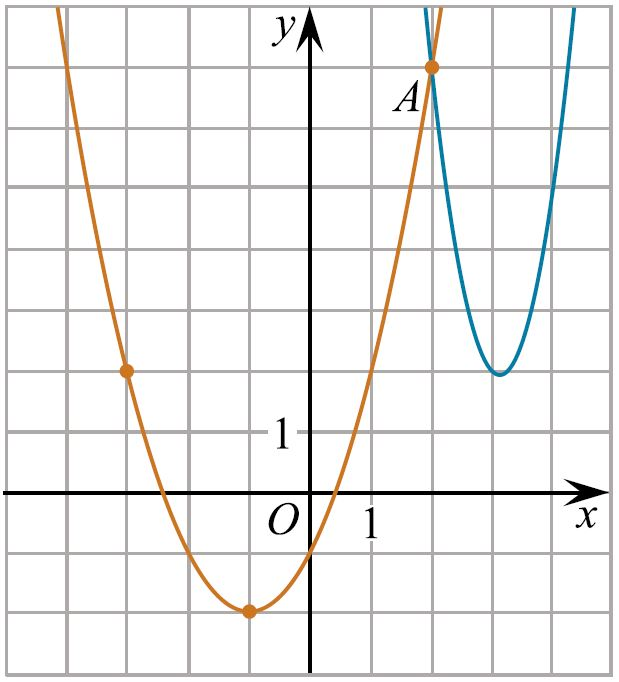
\includegraphics[align=t, width=\linewidth]{../pics/G112M3C1-10}
		%\end{minipage}
		%\item %1 LOGARIFM
		%\begin{minipage}[t]{\bodywidth}
		%	На рисунке изображен график функции \(f(x) = b+\log_ax \). Найдите \(f(32)\).
		%\end{minipage}
		%\hspace{0.02\linewidth}
		%\begin{minipage}[t]{\picwidth}
		%	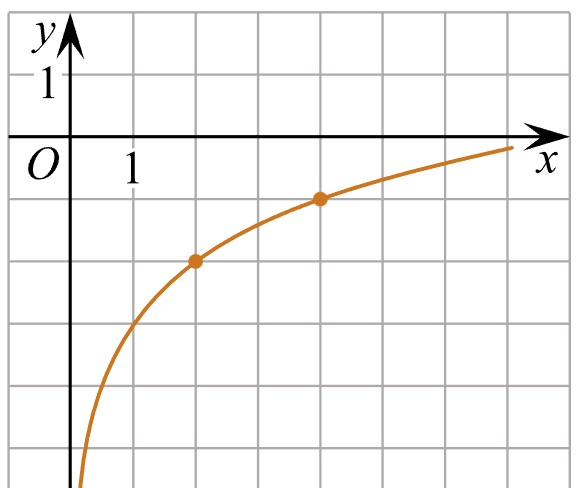
\includegraphics[align=t, width=\linewidth]{../pics/G111M8L1-1}
		%\end{minipage}
		%\item %1 s golovi
		%\begin{minipage}[t]{\bodywidth}
		%	На рисунке изображен график функции \(f(x) = \dfrac{ x^2 }{ a }+bx+c \), где числа \(a, b, c\) --- целые. Найдите значение \(f(3,5)\).
		%\end{minipage}
		%\hspace{0.02\linewidth}
		%\begin{minipage}[t]{\picwidth}
		%	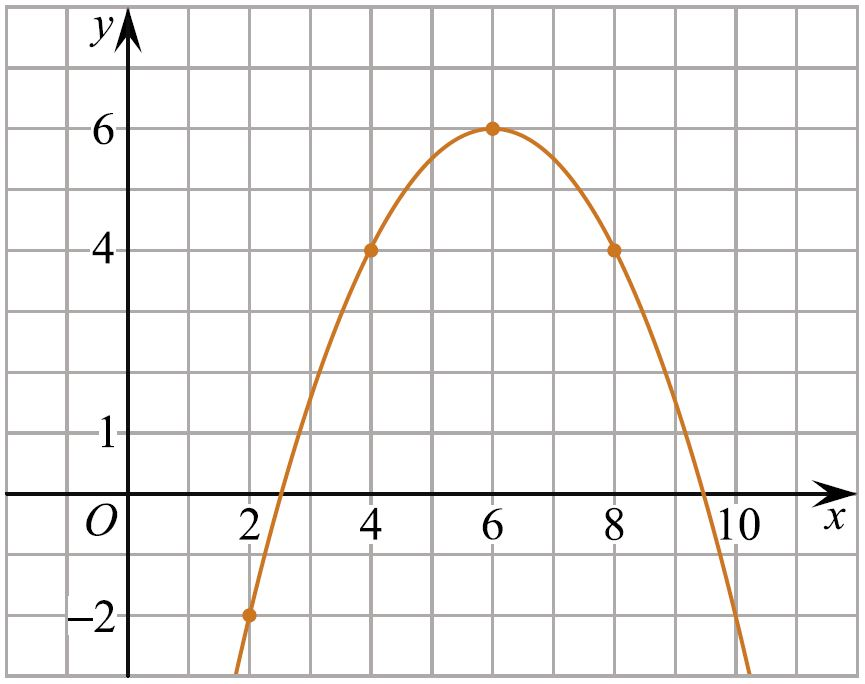
\includegraphics[align=t, width=\linewidth]{../pics/G112M3C1-6}
		%\end{minipage}
		
		
		
		%EGE-1(90g) - 1
		\item В треугольнике \(ABC\) угол \(C\) равен \(90\degree\), \(AC=4,8\), \( \sin A = \dfrac{ 7 }{ 25 } \). Найдите \(AB\).
		%EGE-1(90g) - 4
		\item В треугольнике \(ABC\) угол \(C\) равен \(90\degree\), \(AC=4\), \( \tg A = \dfrac{ 33 }{ 4\sqrt{33} } \). Найдите \(AB\). 
		%n5 cos1
		\item Найдите корни уравнения: \( \cos \dfrac{ \pi(x-7) }{ 3 } = 0,5 \).  В ответ запишите наибольший отрицательный корень.
		%n5 cos3
		\item Найдите корни уравнения: \( \cos \dfrac{ \pi(2x+9) }{ 3 } = \dfrac{ \sqrt{2} }{ 2 } \).  В ответ запишите наибольший отрицательный корень.
		%n5 tg1
		\item Найдите корни уравнения: \( \tg \dfrac{ \pi x }{ 4 } = -1 \).  В ответ запишите наибольший отрицательный корень.
		%n5 tg2
		\item Найдите корни уравнения: \( \tg \dfrac{ \pi (x+2) }{ 3 } = -\sqrt{3} \).  В ответ запишите наибольший отрицательный корень.
		%n5 sin1
		\item Найдите корни уравнения: \( \sin \dfrac{ \pi x }{ 3 } = 0,5 \).  В ответ запишите наименьший положительный корень.
		
		%???chelnokovam5
		\item Вычислить: 
		\begin{tasks}(2)
			\task \( \dfrac{5\cos29\degree}{\sin61\degree} \)
			\task \( -4\sqrt{3}\cos(-750\degree) \)
			\task \( \dfrac{4\cos146\degree}{\cos34\degree} \)
			\task \( 7\tg13\degree\cdot\tg77\degree \)
			\task \( \dfrac{12}{\sin^227\degree+\cos^2207\degree} \)
			\task \( \dfrac{5\sin98\degree}{\sin49\degree\cdot\sin41\degree} \)
			\task \( -50\tg9\degree\cdot\tg81\degree+31 \)
		\end{tasks}
		%?
		\item
		\begin{minipage}[t]{\bodywidth}
			На рисунке изображён график функции \[ f(x)=a \cos{x}+b \] Найдите \(a\).
		\end{minipage}
		\hspace{0.02\linewidth}
		\begin{minipage}[t]{\picwidth}
			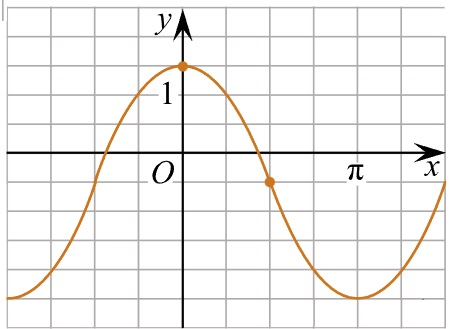
\includegraphics[align=t, width=\linewidth]{\picpath/MECGERM6H3-1}
		\end{minipage}
		%?
		\item
		\begin{minipage}[t]{\bodywidth}
			На рисунке изображён график функции \[ f(x)=a \tg{x}+b \] Найдите \(a\).
		\end{minipage}
		\hspace{0.02\linewidth}
		\begin{minipage}[t]{\picwidth}
			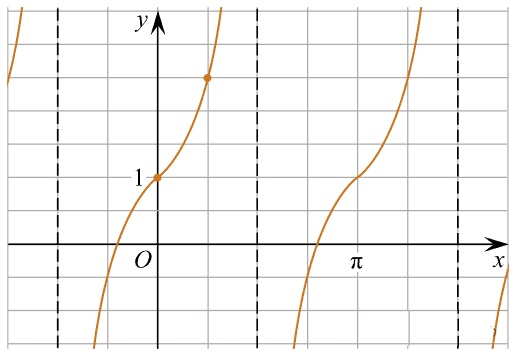
\includegraphics[align=t, width=\linewidth]{\picpath/MECGERM6H3-2}
		\end{minipage}
		%EGE-11 Trigon 1-3
		\item Найдите наибольшее значение функции \[ y=12\cos x + 6\sqrt{3}x - 2 \sqrt{3}x - 2 \sqrt{3} \pi + 6\] на отрезке \( \left[ 0; \dfrac{ \pi }{ 2 } \right]  \).
		\item Найдите наименьшее значение функции \( y=3+\dfrac{ 5\pi }{ 4 }-5x-5\sqrt{2} \cos x\) на отрезке \( \left[ 0; \dfrac{ \pi }{ 2 } \right]  \).
		\item Найдите наибольшее значение функции \( y=5 \cos x - 6x + 4 \) на отрезке \( \left[ -\dfrac{ 3\pi }{ 2 }; 0 \right]  \).
	\end{listofex}
\end{class}
%END_FOLD

%BEGIN_FOLD % ====>>_____ Занятие 2 _____<<====
\begin{class}[number=2]
	\begin{listofex}
		\item Занятие 2
	\end{listofex}
\end{class}
%END_FOLD

%BEGIN_FOLD % ====>>_ Домашняя работа 1 _<<====
\begin{homework}[number=1]
	\begin{listofex}
		\item Домашняя работа 1
	\end{listofex}
\end{homework}
%END_FOLD

%BEGIN_FOLD % ====>>_____ Занятие 3 _____<<====
\begin{class}[number=3]
	\begin{listofex}
		\item Занятие 3 
	\end{listofex}
\end{class}
%END_FOLD

%BEGIN_FOLD % ====>>_____ Занятие 4 _____<<====
\begin{class}[number=4]
	\begin{listofex}
		\item Занятие 4
	\end{listofex}
\end{class}
%END_FOLD

%BEGIN_FOLD % ====>>_ Домашняя работа 2 _<<====
\begin{homework}[number=2]
	\begin{listofex}
		\item Домашняя работа 2
	\end{listofex}
\end{homework}
%END_FOLD

%BEGIN_FOLD % ====>>_____ Занятие 5 _____<<====
\begin{class}[number=5]
	\begin{listofex}
		\item Занятие 5
	\end{listofex}
\end{class}
%END_FOLD

%BEGIN_FOLD % ====>>_____ Занятие 6 _____<<====
\begin{class}[number=6]
	\begin{listofex}
		\item Занятие 6
	\end{listofex}
\end{class}
%END_FOLD

%BEGIN_FOLD % ====>>_ Домашняя работа 3 _<<====
\begin{homework}[number=3]
	\begin{listofex}
		\item Домашняя работа 3
	\end{listofex}
\end{homework}
%END_FOLD

%BEGIN_FOLD % ====>>_____ Занятие 7 _____<<====
\begin{class}[number=7]
	\title{Подготовка к проверочной}
	\begin{listofex}
		\item Занятие 7
	\end{listofex}
\end{class}
%END_FOLD

=%BEGIN_FOLD % ====>>_ Проверочная работа _<<====
\begin{exam}
	\begin{listofex}
		\item Проверочная
	\end{listofex}
\end{exam}
%END_FOLD